\subsection{Implementation}
\label{sect:implementation}

Note: this text and the associated figures are out of date and will be updated.
It is missing all of SMDA.

iPad apps are implemented in the Objective-C language and the Cocoa Touch
application framework. The PathCase apps use the framework to query the database
server and present a scrollabe, zoomable graph view.

Cocoa provides many common facilities such as user interface elements, network
requests, asynchronous blocks of code, and touch operations like panning and
zooming. Core Animation, a subframework, provides rendering capabilities.

Cocoa follows a Model-View-Controller architecture and makes heavy use of the
delegate pattern rather than employing subclasses for custom functionality.
Interface layouts are specified in ``.xib'' files, each of which is associated
with a class. \cite{ios:application-programming-guide}

Core Animation uses the concept of nested layers to allow applications to
efficiently render pieces of a view using different effects and levels of
detail.  \cite{ios:core-animation}

The MAW application is divided into several classes. The relationships between
them are represented in three figures. Figure \ref{fig:maw_components} shows
references between instances. Figure \ref{fig:maw_controlflow} shows the flow of
control in response to events from the event loop. Figure \ref{fig:maw_dataflow}
shows the flow of data between the methods involved in loading and displaying a
graph.

\texttt{PCAppDelegate} handles application-level delegate methods and
notifications from the system.  \texttt{PCGraphViewController}, associated with
\texttt{GraphView.xib}, ties together all user interface elements. There are
currently only two interactive elements, the graph view and the ``Pathways''
button on the toolbar.

The Pathways button causes a popover list of available pathways to be displayed.
This popover is populated by \texttt{PCPathwayListTableController}. When one of
these pathway names is clicked, an event is sent back to
\texttt{PCGraphViewController}, which requests graph data from the PathCase
server. This data is parsed by \texttt{PCGraphModel}, \texttt{PCGraphNode}, and
\texttt{PCGraphEdge} into renderable objects.

The \texttt{PCGraphModel} is attached to a \texttt{PCGraphView} which puts the
graphics data into a series of nested layers and provides it to a
\texttt{UIScrollView}, a Cocoa object which provides panning and zooming.

\onecolumn

\begin{figure}[p]
    \center{
        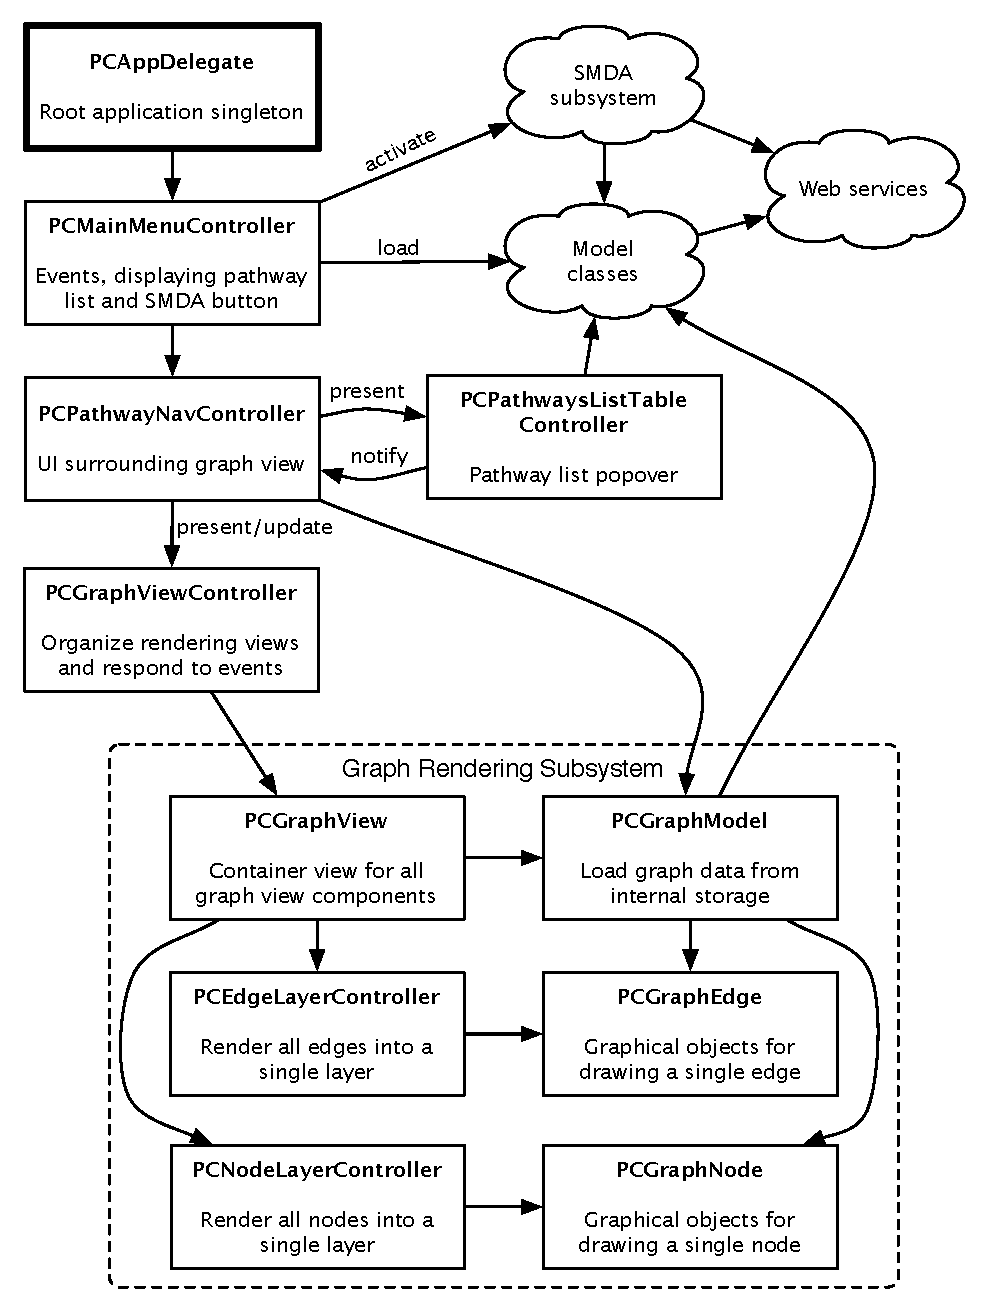
\includegraphics[width=4.5in]{maw/figures/components.pdf}}
    \caption{\label{fig:maw_components} Components of the architecture}
\end{figure}

\begin{figure}[htbp]
    \center{
        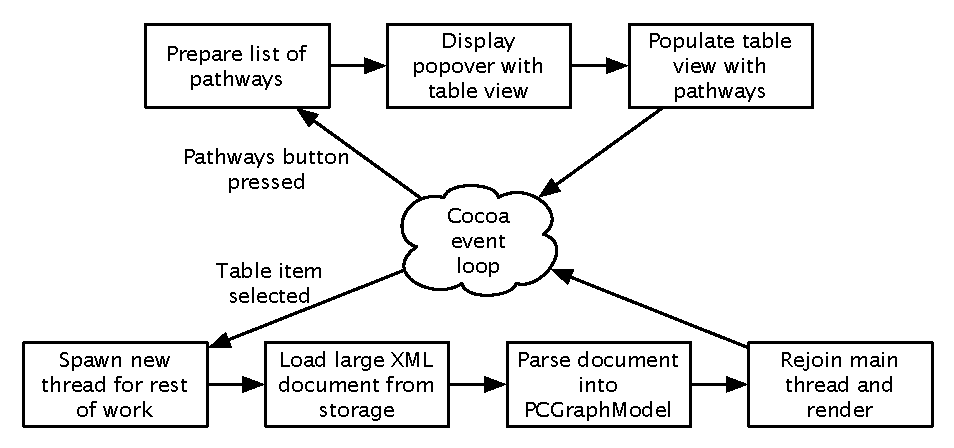
\includegraphics[height=2in]{maw/figures/controlflow.pdf}}
    \caption{\label{fig:maw_controlflow} Control flow for displaying graphs}
\end{figure}

\begin{figure}[thbp]
    \center{
        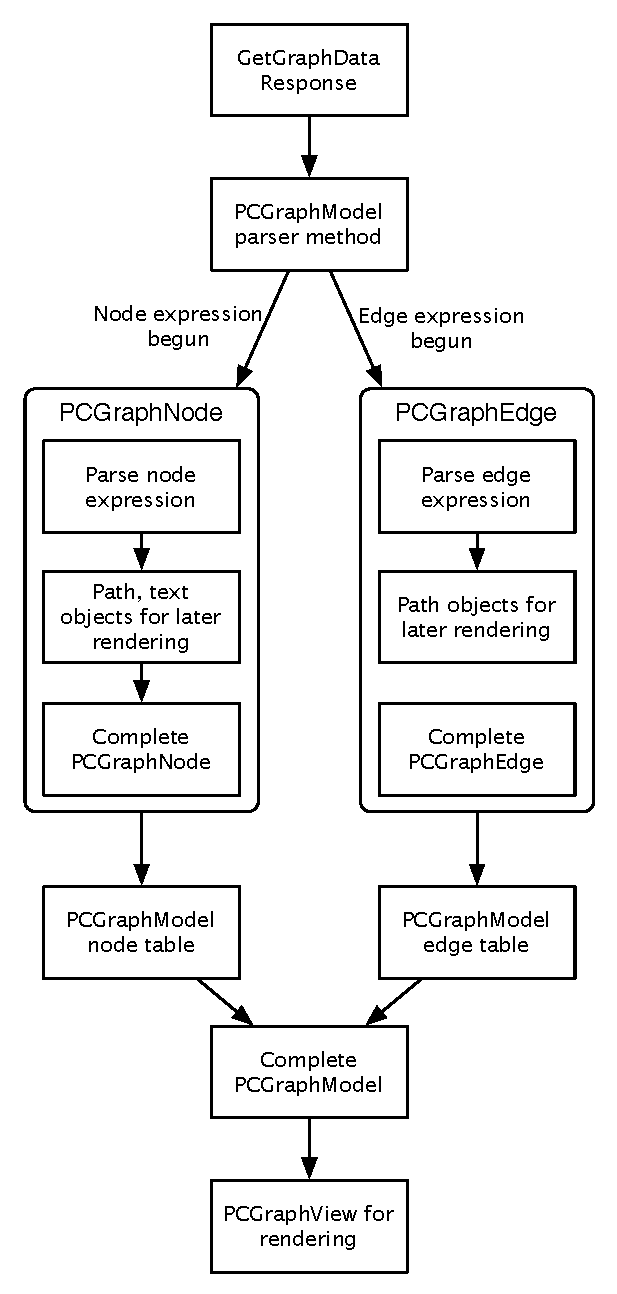
\includegraphics[height=4in]{maw/figures/dataflow.pdf}}
    \caption{\label{fig:maw_dataflow} Data flow for graph data}
\end{figure}

\twocolumn
